% THIS DOCUMENT IS FOLLOWS THE VOLERE TEMPLATE BY Suzanne Robertson and James Robertson
% ONLY THE SECTION HEADINGS ARE PROVIDED
%
% Initial draft from https://github.com/Dieblich/volere
%
% Risks are removed because they are covered by the Hazard Analysis
\documentclass[12pt]{article}

\usepackage{booktabs}
\usepackage{tabularx}
\usepackage{graphicx}
\usepackage{float}
\usepackage{amsmath}
\usepackage{soul}
\usepackage{tikz}

\usepackage{hyperref}
\hypersetup{
    bookmarks=true,         % show bookmarks bar?
      colorlinks=true,      % false: boxed links; true: colored links
    linkcolor=red,          % color of internal links (change box color with linkbordercolor)
    citecolor=green,        % color of links to bibliography
    filecolor=magenta,      % color of file links
    urlcolor=cyan           % color of external links
}

\newcommand{\lips}{\textit{Insert your content here.}}

%% Comments

\usepackage{color}

\newif\ifcomments\commentstrue %displays comments
%\newif\ifcomments\commentsfalse %so that comments do not display

\ifcomments
\newcommand{\authornote}[3]{\textcolor{#1}{[#3 ---#2]}}
\newcommand{\todo}[1]{\textcolor{red}{[TODO: #1]}}
\else
\newcommand{\authornote}[3]{}
\newcommand{\todo}[1]{}
\fi

\newcommand{\wss}[1]{\authornote{blue}{SS}{#1}} 
\newcommand{\plt}[1]{\authornote{magenta}{TPLT}{#1}} %For explanation of the template
\newcommand{\an}[1]{\authornote{cyan}{Author}{#1}}

%% Common Parts

\newcommand{\progname}{Housemates} % PUT YOUR PROGRAM NAME HERE
\newcommand{\authname}{Team \#9, Housemates
\\ Justin Dang - dangj15 
\\ Harris Hamid - hamidh1
\\ Fady Morcos - morcof2 
\\ Rizwan Ahsan - ahsanm7
\\ Sheikh Afsar - afsars} % AUTHOR NAMES                  

\usepackage{hyperref}
    \hypersetup{colorlinks=true, linkcolor=blue, citecolor=blue, filecolor=blue,
                urlcolor=blue, unicode=false}
    \urlstyle{same}
                                


\begin{document}

\title{Software Requirements Specification for \progname \\ (Volere)}
\author{\authname}
\date{\today}
	
\maketitle

~\newpage

\pagenumbering{roman}

\tableofcontents

~\newpage

\section*{Revision History}

\begin{tabularx}{\textwidth}{p{3cm}p{2cm}X}
\toprule {\textbf{Date}} & {\textbf{Version}} & {\textbf{Notes}}\\
\midrule
6 October 2023 & 1.0 & Initial Draft\\
2 April 2024 & 1.1 & First Revision \\
\bottomrule
\end{tabularx}

~\\

~\newpage

\section{Template and Changes}

This SRS follows the Volere SRS template. A traceability section was added to ensure that the requirements of \progname{} are traceable with the other \progname{} documentation.  Some sections were removed from this document if they didn't apply to the SRS of \progname{} (e.g. Open Issues, New Problems, User Documentation and Training, Waiting Room, etc.). 

\section{Naming Conventions and Terminology}
\subsection{Glossary of all terms used by stakeholders}
\begin{itemize}
    \item Housemates: The main application being developed.
    \item Roommates: People living in the same household.
    \item Group: Users who share common expenses, tasks or schedule for a particular purpose.
\end{itemize}
\section{Purpose of the Project}
\subsection{User Business}

With the ongoing affordable housing shortage in Canada many people have been forced to find roommates in order to have a place to live in. This is especially common at universities like McMaster where its extremely common to have roommates while in student housing. While having roommates may help ease financial pressures it can lead to a lot of stress in dealing with them. These stresses can include things like dealing with splitting household tasks and grocery costs. An application that helps deal with these common stresses in the roommate life would make it more convenient  for the roommates to live together and overall simplify their lives.

\subsection{Goals of the Project}

\begin{center}
\begin{tabular}{|p{6cm}|p{6cm}|}
\hline
\textbf{Goals} & \textbf{Importance}\\
\hline The application will have a straightforward and user-friendly interface that is simple to use for all users, regardless of technical ability. & This allows first time users to be interested in our product and a good experience with the overall product. \\
\hline
The application will simplify household tasks through a task management system. & This allows streamlining the allocation of chores which in return will reduce conflicts and misunderstandings between roommates. \\
\hline
The application will streamline expense sharing through a bill management system. & This makes it possible for roommates to monitor their expenditure and prevent overspending. Additionally, it encourages each person to make a fair financial contribution. \\
\hline
The application will have a scheduling system that will allow for users to schedule quiet hours & This allows users to focus on their work, sleep, or studies without any interruption. \\
\hline
The application will have a calendar to see scheduled events & This allows users to coordinate their schedules and help them in managing their time in a better way. \\
\hline
\end{tabular}
\end{center}

\section{Stakeholders}
% \subsection{Client}

% N/A

\subsection{Customer}

\begin{itemize}
    \item People with roommates: People with roommates are the primary stakeholders of this application. They can use the application to better simplify life with roommates. As such they will have the greatest influence out of the stakeholders on the requirements of the application during the development process.
\end{itemize}

\subsection{Other Stakeholders}

\begin{itemize}
  \item Landlords / Property Manager / Housing Association: Landlords would be a secondary stakeholder for the application. Landlords might be interested in using an application like this for their tenants so that they will better be able to communicate with them with respects to household tasks that are required. As such, they might play a minor role on determining the requirements of the application during the design process.
  \item Families: Families can also benefit from the app to have a centralized place for all household matters. They can distribute chores evenly and keep track of bills. It promotes talking openly and encourages users to be more responsible about household duties and bills.
\end{itemize}

\subsection{Hands-On Users of the Project}

\begin{itemize}
    \item People with roommates
    \item Landlords / Property Manager / Housing Association
    \item Families
\end{itemize}

\subsection{Personas}
Andrew is a student at McMaster University. He lives off-campus in student housing with four other roommates. He and his roommates have to buy groceries and supplies for the house. They also have to do various household chores and pay for utilities and internet. Sometimes Andrew and his roommates have trouble communicating with one another on this. Additionally, Andrew gets annoyed when his roommates decide to have a party the day before Andrew has an exam.

\subsection{Priorities Assigned to Users}

The primary stakeholders for this project are people with roommates and as such they will have the highest priority during the development process. The other stakeholders will be considered during the development process, but overall will have a lower priority.

\subsection{User Participation}

During the development process we plan to test the application with the stakeholders described above. Their feedback will help improve the application to better fit their needs.

\subsection{Maintenance Users and Service Technicians}

During the development of this project the project will be maintained by the development team.

\section{Mandated Constraints}


\subsection{Implementation Environment of the Current System}

The expected environment for this application will be a browser-supported device providing a user-friendly and intuitive application that is really simple to use. With goals of expanding as a mobile app, so that we can cater to a much diverse user base using mobiles with Android or iOS. Users would then have the convenience to access the solution/product on any device they want that suits their needs. 





\subsection{Anticipated Workplace Environment}
The anticipated workplace environment for this application is in users' homes since this application deals with roommates. However, as this app is also on mobile devices there could be a wide variety of places where this application could be used.

\subsection{Schedule Constraints}
This project is being developed from September 2023 - April 2024.
\subsection{Budget Constraints}
This project has a budget constraint of \$750.



\section{Assumptions}
% \subsection{Relevant Facts}
% \lips
% \subsection{Business Rules}
% N/A
\begin{itemize}
    \item The users of this application are expected to have a basic understanding of how to access a website through a browser.
\end{itemize}

% \section{The Scope of the Work}
% \subsection{The Current Situation}
% \lips
% \subsection{The Context of the Work}
% \lips
% \subsection{Work Partitioning}
% \lips
% \subsection{Specifying a Business Use Case (BUC)}
% \lips
% Don't think we neeed this part yet

% \section{Business Data Model and Data Dictionary}
% \subsection{Business Data Model}
% \lips
% % \subsection{Data Dictionary}
% % \lips
% % Dont think we need this part yet

\section{Scope}
\subsection{Product Context}
The following diagram depicts the main application interacting with external systems and users and the relation between them in terms of data flow.

\subsubsection*{Database:}This acts as the storage for all the information that the application will receive, process and save.

\subsubsection*{Housemates App:} This is the main software application that the user will interact with to achieve their goals by making requests to different components of the application.

\subsubsection*{App User:} This is the user interacting with the Housemates app in order to trigger events to request for information to be displayed.
\begin{figure}[H]
    \centering
	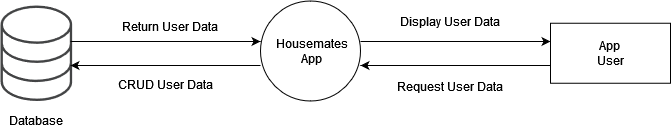
\includegraphics[width=15cm]{ContextDiagram.png}
	\caption{Context Diagram}
 \label{}
\end{figure}
\subsection{Individual Product Use Cases (PUC's)}
\begin{itemize}
    \item[PUC1:]
        \begin{itemize}
            \item \textbf{\textit{Title}: Create user account}
            \item \textit{Precondition}: User does not have existing account.
            \item \textit{Trigger}: User selects option to create new account.
            \item \textit{Description}:Allows user to provide necessary information (such as name, email, password) to create a new account within the system.
    \end{itemize}

    \item[PUC2:]
        \begin{itemize}
            \item \textbf{\textit{Title}: Log in}
            \item \textit{Precondition}: User has an existing account.
            \item \textit{Trigger}: User enters their information and selects the log in option.
            \item \textit{Description}: Allows user to authenticate and access their existing account.
    \end{itemize}

    \item[PUC3:]
        \begin{itemize}
            \item \textbf{\textit{Title}: Add household chores}
            \item \textit{Precondition}: User is logged in and is present in a group.
            \item \textit{Trigger}: User selects the option to add a new household chore.
            \item \textit{Description}: Enables users to create a new household chore with details like name, description, frequency and assign it.
    \end{itemize}

    \item[PUC4:]
        \begin{itemize}
            \item \textbf{\textit{Title}: Edit household chores}
            \item \textit{Precondition}: User is logged in and has existing household chore.
            \item \textit{Trigger}: User selects the option to edit an existing household chore.
            \item \textit{Description}: Allows users to modify details of an existing household chore, such as its name, description, frequency and assignee.
    \end{itemize}

    \item[PUC5:]
        \begin{itemize}
            \item \textbf{\textit{Title}: Remove household chores}
            \item \textit{Precondition}: User is logged in and has existing household chore.
            \item \textit{Trigger}: User selects the option to delete an existing household chore.
            \item \textit{Description}: Allows users to remove a household chore that is no longer required.
    \end{itemize}

    \item[PUC6:]
        \begin{itemize}
            \item \textbf{\textit{Title}: Marking completion of household chores}
            \item \textit{Precondition}: User is logged in and has existing household chore.
            \item \textit{Trigger}: User selects the option to mark a household chore as completed.
            \item \textit{Description}: Allows users to mark off a specific household chore and track that it has been successfully completed.
    \end{itemize}

    \item[PUC7:]
        \begin{itemize}
            \item \textbf{\textit{Title}: Add expense}
            \item \textit{Precondition}: User is logged in.
            \item \textit{Trigger}: User selects the option to add a new household expense.
            \item \textit{Description}: Enables users to record a new expense between all or specific roommates, including details like item name, cost, date of purchase, etc.
    \end{itemize}

    \item[PUC8:]
        \begin{itemize}
            \item \textbf{\textit{Title}: Edit expense}
            \item \textit{Precondition}: User is logged in and has existing existing expense.
            \item \textit{Trigger}: User selects the option to edit an existing expense.
            \item \textit{Description}: Allows users to modify details of an existing expense.
    \end{itemize}

    \item[PUC9:]
        \begin{itemize}
            \item \textbf{\textit{Title}: Delete expense}
            \item \textit{Precondition}: User is logged in and has existing expense.
            \item \textit{Trigger}: User selects the option to delete an existing expense.
            \item \textit{Description}: Enables users to remove an expense that is no longer relevant or was added by mistake.
    \end{itemize}

    \item[PUC10:]
        \begin{itemize}
            \item \textbf{\textit{Title}: Mark expense as settled}
            \item \textit{Precondition}: User is logged in and has existing household chore.
            \item \textit{Trigger}: User selects the option to mark a household chore as completed.
            \item \textit{Description}: Allows users to mark off a specific household chore and track that it has been successfully completed.
    \end{itemize}

    \item[PUC11:]
        \begin{itemize}
            \item \textbf{\textit{Title}: View task list}
            \item \textit{Precondition}: User is logged in and has existing tasks/chores.
            \item \textit{Trigger}: User selects the option to view the task list.
            \item \textit{Description}: Displays a list of all current tasks for the user's household.
    \end{itemize}

    \item[PUC12:]
        \begin{itemize}
            \item \textbf{\textit{Title}: View expense summary}
            \item \textit{Precondition}: User is logged in and has existing expenses.
            \item \textit{Trigger}: User selects the option to view the expense summary.
            \item \textit{Description}: Displays an overview of shared expenses and individual contributions.
    \end{itemize}

    \item[PUC13:]
        \begin{itemize}
            \item \textbf{\textit{Title}: View calendar}
            \item \textit{Precondition}: User is logged in.
            \item \textit{Trigger}: User selects the option to view the calendar.
            \item \textit{Description}: Displays a calendar with scheduled events, tasks, and quiet hours.
    \end{itemize}

    \item[PUC14:]
        \begin{itemize}
            \item \textbf{\textit{Title}: Set quiet hours}
            \item \textit{Precondition}: User is logged in and has roommates added.
            \item \textit{Trigger}: User selects the option to set quiet hours.
            \item \textit{Description}: Allows users to define specific time periods for quiet hours in the living space.
    \end{itemize}

    \item[PUC15:]
        \begin{itemize}
            \item \textbf{\textit{Title}: Log out}
            \item \textit{Precondition}: User is logged.
            \item \textit{Trigger}: User selects the option to log out.
            \item \textit{Description}: Allows a logged-in user to securely log out of their account, ending their current session.
    \end{itemize}


\end{itemize}

\subsection{Product Use Case Diagram}
\begin{figure}[H]
    \centering
	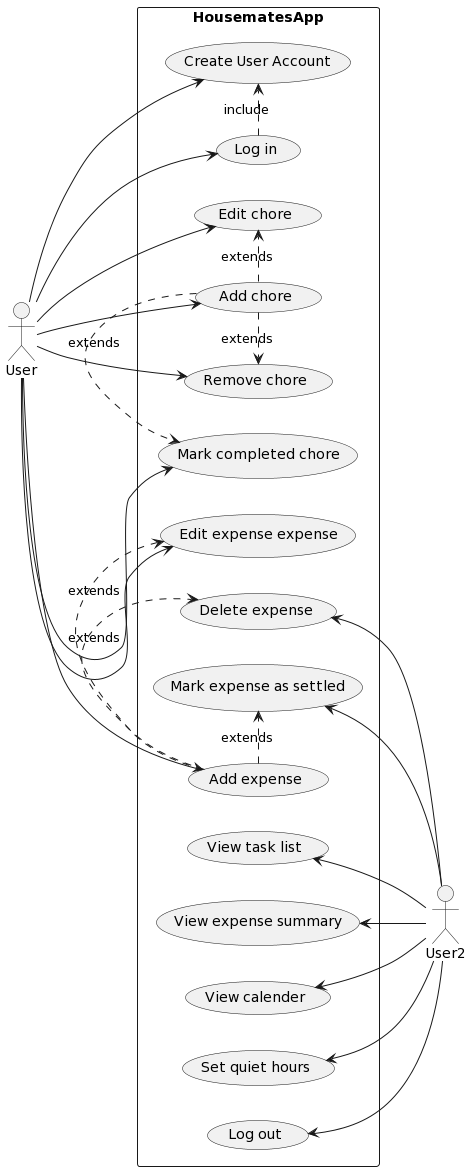
\includegraphics[width=6.5cm]{UseCase.png}
	\caption{Usecase Diagram}
 \label{}
\end{figure}




\section{Functional Requirements}
\subsection{Task Management System}
\noindent \begin{itemize}
    \item[TM1:] 
    \begin{itemize}
        \item \textit{Description}: User tasks will be displayed in task management page.
        \item \textit{Rationale}: This is to be able to clearly view the tasks which the user must complete.
    \end{itemize}
    \item[TM2:] 
    \begin{itemize}
    \item \textit{Description}: Users are able to create new tasks.
    \item \textit{Rationale}: Users need to be able to add new tasks as needed.
    \item \textit{Fit Criterion}: User able to see task added to bill management page.
    
    \end{itemize}
    \item[TM3:]
    \begin{itemize}
    \item \textit{Description}: Users are able to assign tasks to roommates.
    \item \textit{Rationale}: This feature enables users to divide tasks among roommates.
    \item \textit{Fit Criterion}: Other users are able to see task on their end.
    
    \end{itemize}
    \item[TM4:]
    \begin{itemize}
    \item \textit{Description}: Users can mark tasks as completed.
    \item \textit{Rationale}: Users need to be allowed to track the progress of tasks and mark them as completed when they are done.
    \item \textit{Fit Criterion}: Task is removed from current tasks and moved to completed tasks.
    \end{itemize}
    
\end{itemize}
\subsection{Bill Management System}
\noindent \begin{itemize}
    \item[BM1:] 
    \begin{itemize}
        \item \textit{Description}: Users are able to create a new bill.
        \item \textit{Rationale}: This requirement allows users to create new bills as needed.
    \end{itemize}
    \item[BM2:] 
    \begin{itemize}
        \item \textit{Description}: Users are able to assign bill to a roommate and split it amongst them evenly.
        \item \textit{Rationale}: This functionality will allow users to keep track of bill splitting easily.
        \item \textit{Fit Criterion}: 
        \begin{enumerate}
            \item The bill amount is correctly split evenly amongst the roommates.
            \item The total bill amount is shown on the screen and the amount required to pay by each roommate is displayed correctly.
        \end{enumerate}
    \end{itemize}
    \item[BM3:] 
    \begin{itemize}
        \item \textit{Description}: Users are able to modify already inputted bill details 
        \item \textit{Rationale}: This requirement allows users to modify any information on the bill for any correction or changes.
        \item \textit{Fit Criterion}: Users can view and edit any bill on the page and the changes are saved and reflected correctly on the system.
    \end{itemize}
    \item[BM4:] 
    \begin{itemize}
        \item \textit{Description}: Users are able to categorize the bills.
        \item \textit{Rationale}: This requirements makes it easier for users to differentiate and organize their expenses.
    \end{itemize}
    \item[BM5:] 
    \begin{itemize}
        \item \textit{Description}: Users are able to keep track of which bills have been paid off.
        \item \textit{Rationale}: This requirement will allow users to keep track of their payments.
        \item \textit{Fit Criterion}: 
        \begin{enumerate}
            \item Users can mark any bill they paid off and the system keeps a record of the history.
        \end{enumerate}
    \end{itemize}
    \item[BM6:] 
    \begin{itemize}
        \item \textit{Description}: Users are able to assign bill to a roommate and split it amongst them unevenly.
        \item \textit{Rationale}: This functionality will allow users to split unevenly if required. E.g. Splitting a dinner bill where each user ordered different items with different prices.
        \item \textit{Fit Criterion}: 
        \begin{enumerate}
            \item The bill amount is correctly split amongst the roommates.
            \item The total bill amount is shown on the screen and the amount required to pay by each roommate is displayed correctly.
        \end{enumerate}
    \end{itemize}
    \item[BM7:] 
    \begin{itemize}
        \item \textit{Description}: Users are able to settle expenses from bills.
        \item \textit{Rationale}: This functionality will allow users to remove the expense after they paid it.
        \item \textit{Fit Criterion}: 
        \begin{enumerate}
            \item Once their portion of the bill is paid off the it should show on screen that the amount the user owes for the bill should be 0.
        \end{enumerate}
    \end{itemize}
\end{itemize}



\subsection{Scheduling System}
\noindent \begin{itemize}
    \item[SS1: ]
\begin{itemize}
    \item \textit{Description}: Users are able to create new events and schedule them within the scheduling feature.
    \item \textit{Rationale}: This functionality allows users to plan and coordinate activities efficiently.
    \item \textit{Fit Criterion}: Assigned users are able to see event on scheduling page.
\end{itemize}

\item[SS2: ]
\begin{itemize}
    \item \textit{Description}: Users can view all the events scheduled by other users on their calendar within the scheduling feature.
    \item \textit{Rationale}: Event visibility ensures that all users are aware of shared activities and can plan accordingly.
    \item \textit{Fit Criterion}: Users can clearly see and distinguish between their personal events and shared user events on the calendar.
\end{itemize}
    
\end{itemize}
\subsection{Account System}
\noindent \begin{itemize}
    \item[AS1:] 
    \begin{itemize}
        \item \textit{Description}: Users can create new account by providing their personal information.
        \item \textit{Rationale}: This requirement is essential to allow new users to use the product and personalize their experience within the app.
        \item \textit{Fit Criterion}: The system should allow successful registration of users when they provide valid information
    \end{itemize}
    \item[AS2:] 
    \begin{itemize}
        \item \textit{Description}: Users are able to log in to the system by providing their email address and password.
        \item \textit{Rationale}: This requirement ensures that only authorized users are able to access their accounts and the features available in the app.
        \item \textit{Fit Criterion}: 
        \begin{enumerate}
            \item Users will be able to successfully log in to the app provided they give valid credentials
            \item Users will be unable to log in if they provide invalid credentials and appropriate error message will be shown.
        \end{enumerate}
    \end{itemize}
    \item[AS3:] 
    \begin{itemize}
        \item \textit{Description}: Users are able to update their profile information.
        \item \textit{Rationale}: This requirement will allow user to change their information when they see fit.
        \item \textit{Fit Criterion}: Changes made in the profile section should be updated and reflected properly in the app.
    \end{itemize}
    \item[AS4:] 
    \begin{itemize}
        \item \textit{Description}: Users are able to remove their account from the system.
        \item \textit{Rationale}: Users should be given the option to have control of their own account.
        \item \textit{Fit Criterion}: 
        \begin{enumerate}
            \item Users can temporarily deactivate their account and reactivate them.
            \item Users can permanently delete their account.
        \end{enumerate}
    \end{itemize}
    \item[AS5:] 
   \begin{itemize} \st{
        \item \textit{Description}: Users are able to recover their account in case of forgetting their log in information
        \item \textit{Rationale}: This requirement allows users a way to recover their account and seek support.
        \item \textit{Fit Criterion}: Users are able to click a "Forgot Password" button if they forgot their password which sends an email to their provided email address.}
    \end{itemize}
\end{itemize}
\subsection{Formal Specification of Bill Management System}

A critical aspect of this project involves calculating expenses associated to every roommate. In order to represent all bills and expense associated to every roommate in an accurate and timely fashion, we will formally represent this system using Module Interface Specification. \\

Let:

\begin{itemize}
    \item $I$ be the set of all individual items.
    \item $U$ be the set of all users. 
    \item $C$ be the cost associated with each item.
    \item $S$ be a function that maps an item to its sharers.
    \item $P$ be a function that maps an item to its payment division.
\end{itemize}

\subsubsection*{Individual Costs}

For each item $i$ in $I$, there is a cost $c$ associated with it. Formally:

\[
C: I \rightarrow R^+
\]

This function $C$ maps every item $i$ to its positive cost $c$.

\subsubsection*{Sharers of Costs}

For each item $i$, there's a subset of users $U_i \subseteq U$ who share its cost. The function $S$ determines which users are responsible for which items:

\[
S: I \rightarrow 2^U
\]

Here, $2^U$ represents the power set of $U$, denoting all possible subsets of users. Not all users necessarily owe an amount.

\subsubsection*{Payment Division}

The function $P$ assigns a portion of the item's cost to each user:

\[
P: I \times U \rightarrow R^+
\]

This means for each item $i$ and user $u$ in $U_i$, $P(i, u)$ returns the amount $u$ owes for $i$. If a user $u$ does not share the cost of some item $i$, that is $u \not\in S(i)$, then $P(i, u) = 0$.

\subsubsection*{Constraints}

\subsubsection*{Total Payment}

The total amount paid by all users for an item must equal the cost of that item:

\[
\forall i \in I: \sum_{u \in U} P(i, u) = C(i)
\]

\subsubsection*{Non-negative Payment}

No user can owe a negative amount:

\[
\forall i \in I, \forall u \in U: P(i, u) \geq 0
\]

\subsubsection*{Overall User Expense}

The total amount owed by a user for all items is:

\[
\text{Expense}: U \rightarrow R^+
\]

\[
\text{Expense}(u) = \sum_{i \in I} P(i, u)
\]


\section{Look and Feel Requirements}
\subsection{Appearance Requirements}
\noindent \begin{itemize}
    \item[LF-A1:] 
    \begin{itemize}
        \item \textit{Description}: The application should have a modern minimalist user interface.
        \item \textit{Rationale}: A minimalist user interface design will allow users to intuitively use the application.
        \item \textit{Fit Criterion}: The interface follows the minimalist design principles in \href{https://m3.material.io/foundations}{Google's material design guidelines}. 
    \end{itemize}
\end{itemize}

\subsection{Style Requirements}


\noindent \begin{itemize}
    \item[LF-S1:] 
    \begin{itemize}
        \item \textit{Description}: All pages in the application must follow a similar user interface
        \item \textit{Rationale}: This allows for consistency of style and less ambiguity.
        \item \textit{Fit Criterion}: During beta testing, potential users able to determine whether pages looks are consistent.
    \end{itemize}
\end{itemize}

\section{Usability and Humanity Requirements}
\subsection{Ease of Use Requirements}

\noindent \begin{itemize}
    \item[UH-E1:] 
    \begin{itemize}
        \item \textit{Description}: The application should be easy to navigate.
        \item \textit{Rationale}: Users of the application should able to reach the main features of the application clearly.
        \item \textit{Fit Criterion}: Users of the application should be able to reach the main features of the application within 5 clicks/taps.
    \end{itemize}
\end{itemize}

\subsection{Personalization and Internationalization Requirements}
\noindent \begin{itemize}
    \item[UH-P1:] 
    \begin{itemize}
        \item \textit{Description}: The application will use Canadian English as its primary language.
        \item \textit{Rationale}: Most of the target audience of the application speak English.
        \item \textit{Fit Criterion}: The application uses Canadian English when released.
    \end{itemize}
\end{itemize}

\subsection{Learning Requirements}
\noindent \begin{itemize}
    \item[UH-L1:] 
    \begin{itemize}
        \item \textit{Description}: Users of the application should be able to quickly learn how to use it.
        \item \textit{Rationale}: The application should be easy to learn.
        \item \textit{Fit Criterion}: During testing a user should able to use all of the features of the application within the first 30 minutes of first opening the application.
    \end{itemize}
\end{itemize}

\subsection{Accessibility Requirements}
\noindent \begin{itemize}
    \item[UH-A1:] 
        \begin{itemize}
            \item \textit{Description}: The application should be usable by partially sighted users.
            \item \textit{Rationale}: Accessibility accommodations will allow the app to reach a larger target audience.
            \item \textit{Fit Criterion}: The application uses the various \href{https://support.google.com/accessibility/android/answer/6006564?hl=en}{android accessibility features.}
        \end{itemize}
\end{itemize}

\section{Performance Requirements}
\subsection{Speed and Latency Requirements}
\noindent \begin{itemize}
    \item[P-SL1:] 
        \begin{itemize}
            \item \textit{Description}: The application should respond to user interactions quickly.
            \item \textit{Rationale}: Users should feel the app is responsive.
            \item \textit{Fit Criterion}: The application should respond to user input within 0.5 seconds.
        \end{itemize}
\end{itemize}


% \noindent \begin{itemize}
%     \item[P-SC1:] 
%         \begin{itemize}
%            \item \textit{Description}: 
%             \item \textit{Rationale}: 
%             \item \textit{Fit Criterion}: 
%         \end{itemize}
% \end{itemize}
\subsection{Precision or Accuracy Requirements}
\noindent \begin{itemize}
    \item[P-PA1:] 
        \begin{itemize}
            \item \textit{Description}: All monetary information (e.g. bill amounts) will be accurate to two decimal places. 
            \item \textit{Rationale}: Information from cost-splitting system should be accurate.
            \item \textit{Fit Criterion}: During testing costs will be correctly rounded to two decimal places.
        \end{itemize}
\end{itemize}
\subsection{Robustness or Fault-Tolerance Requirements}
\noindent \begin{itemize}
    \item[P-RFT1:] 
        \begin{itemize}
            \item \textit{Description}: The application should continue to operate locally if it loses connection to the server.
            \item \textit{Rationale}: Users may temporarily lose connection to the application servers during use.
            \item \textit{Fit Criterion}: The application should continue to function for 10 minutes after losing connection to application servers. Additionally it should function as normal when connection is resumed.
        \end{itemize}
\end{itemize}
\subsection{Capacity Requirements}
\noindent \begin{itemize}
    \item[P-C1:] 
        \begin{itemize}
            \item \textit{Description}: The application should be able to handle 100 simultaneous users.
            \item \textit{Rationale}: The application should be handle a lot of users using it at the same time.
            \item \textit{Fit Criterion}: During testing the application should handle 100 simultaneous users.
        \end{itemize}
\end{itemize}
\subsection{Scalability or Extensibility Requirements}


\noindent \begin{itemize}
    \item[P-SE1:] 
        \begin{itemize}
            \item \textit{Description}: The application should horizontally scale when the number of users increase.
            \item \textit{Rationale}: To ensure consistent performance among users.
            \item \textit{Fit Criterion}: Use performance testing tool to check response times.
        \end{itemize}
\end{itemize}



\section{Operational and Environmental Requirements}
\subsection{Expected Physical Environment}
\noindent \begin{itemize}
    \item[OE-PE1:] 
        \begin{itemize}
            \item \textit{Description}: The system will be able to run on devices that support a browser.
            \item \textit{Rationale}: Being available on such devices will allow the application to reach a wide target audience.
            \item \textit{Fit Criterion}: The application is able to run on phones, tablets and PCs.
        \end{itemize}
\end{itemize}


% \noindent \begin{itemize}
%     \item[OE-I1:] 
%         \begin{itemize}
%             \item \textit{Description}: 
%             \item \textit{Rationale}: 
%             \item \textit{Fit Criterion}: 
%         \end{itemize}
% \end{itemize}
\subsection{Productization Requirements}
\noindent \begin{itemize}
    \item[OE-PR1:] 
        \begin{itemize}
            \item \textit{Description}: The application should be deployed on a server.
            \item \textit{Rationale}: Being deployed entails that anyone on the internet can use the application.
            \item \textit{Fit Criterion}: The application is accessible through its unique URL.
        \end{itemize}
\end{itemize}


% \noindent \begin{itemize}
%     \item[OE-R1:] 
%         \begin{itemize}
%            \item \textit{Description}: 
%             \item \textit{Rationale}: 
%             \item \textit{Fit Criterion}: 
%         \end{itemize}
% \end{itemize}

\section{Maintainability and Support Requirements}
\subsection{Maintenance Requirements}
\noindent \begin{itemize}
    \item[M-M1:] 
        \begin{itemize}
            \item \textit{Description}:  The development process for the application should be well documented.
            \item \textit{Rationale}: Proper documentation will ensure that the system will be maintainable in the future.
            \item \textit{Fit Criterion}: The documentation should contain an up to date Problem Statement, Development Plan, SRS, Hazard analysis, Software Design, Software testing, etc. documents. 
        \end{itemize}
\end{itemize}


\section{Security Requirements}
\subsection{Access Requirements}
\noindent \begin{itemize}
    \item[S-A1:] 
        \begin{itemize}
           \item \textit{Description}: The application should only allow system administrators to access user data.
            \item \textit{Rationale}: User data should remain private unless necessary.
            \item \textit{Fit Criterion}: In the application user data will not be accessible by other users.
        \end{itemize}
\end{itemize}
\subsection{Integrity Requirements}
\noindent \begin{itemize}
    \item[S-IN1:] 
        \begin{itemize}
           \item \textit{Description}: The application should prevent incorrect data from being introduced.
            \item \textit{Rationale}: Incorrect data being introduced into the database could be used to attack the database.
            \item \textit{Fit Criterion}: In the application users can't introduce incorrect data in any entry fields.
        \end{itemize}
\end{itemize}
\subsection{Privacy Requirements}
\noindent \begin{itemize}
    \item[S-P1:] 
        \begin{itemize}
            \item \textit{Description}: The application should make the user aware of its information collection policy before collecting data from them.
            \item \textit{Rationale}: Users should be aware of any personal data collected and the reason why it is collected.
            \item \textit{Fit Criterion}: The application notifies users on first launch the information collection policy.
        \end{itemize}
\end{itemize}


\section{Cultural Requirements}
\subsection{Neutrality Requirements}
\noindent \begin{itemize}
    \item[CR-N1:] 
        \begin{itemize}
            \item \textit{Description}: The user interface must not be indicative to any particular culture.
            \item \textit{Rationale}: The symbols or colors in the app may offend some users.
            \item \textit{Fit Criterion}: During field testing, users from different backgrounds can approve of the design.
        \end{itemize}
\end{itemize}

\section{Compliance Requirements}

\subsection{Standards Compliance Requirements}
\noindent \begin{itemize}
    \item[C-SC1:] 
        \begin{itemize}
            \item \textit{Description}: The application should inform users beforehand about the data being collected and stored from them.
            \item \textit{Rationale}: This allows for transparency between provider and users.
            \item \textit{Fit Criterion}: A terms and condition page is displayed before they are able to interact with the application.
        \end{itemize}
\end{itemize}


\section{Off-the-Shelf Solutions}
\subsection{Ready-Made Products}
For off the shelf solutions there are many individual cost splitting/chore splitting apps available on the App store/Google Play Store. However these apps don't capture the functionality of both a cost-management and chore-management system.\\

Cost-splitting
\begin{itemize}
    \item \href{https://play.google.com/store/apps/details?id=splid.teamturtle.com.splid&hl=en&gl=US}{Splid}
    \item \href{https://www.splitwise.com/}{Splitwise}
    \item \href{https://www.tricount.com/en/mobile}{Tricount}
    \item \href{https://splitser.com/}{Splitser}
    \item \href{https://settleup.io/}{Settle Up}
\end{itemize}



Chore-Splitting
\begin{itemize}
    \item \href{https://todyapp.com/}{Tody}
    \item \href{https://nipto.app/}{Nipto}
    \item \href{https://sweepy.app/}{Sweepy}
    \item \href{https://play.google.com/store/apps/details?id=com.remedy.chap&hl=en&gl=US}{Chap}
    \item \href{https://play.google.com/store/apps/details?id=flatify.com.flatify&pcampaignid=web_share}{Flatify}
\end{itemize}



% \subsection{Effects on the Current Environment}
% \lips
% \subsection{Effects on the Installed Systems}
% \lips
% \subsection{Potential User Problems}
% \lips
% \subsection{Limitations in the Anticipated Implementation Environment That May
% Inhibit the New Product}
% \lips
% \subsection{Follow-Up Problems}
% \lips

\section{Tasks}
\subsection{Project Planning}

\begin{center}
\begin{tabular}{ |c|c| } 
\hline
\textbf{Deliverable} & \textbf{Deadline} \\ 
 \hline
 Problem Statement, POC Plan, Development Plan & September 25 \\ 
 Requirements Document Revision 0  & October 6 \\
Hazard Analysis 0 & October 20  \\ 
 V\&V Plan Revision 0 & November 3 \\ 
Proof of Concept Demonstration & November 13--24 \\
Design Document Revision 0 & January 17 \\
Revision 0 Demonstration & February 5--February 16\\
V\&V Report Revision 0 & March 6 \\
Final Demonstration (Revision 1) & March 18--March 29 \\
EXPO Demonstration & April TBD \\
Final Documentation (Revision 1) & April 4 \\
 \hline
\end{tabular}
\end{center}

\subsection{Planning of the Development Phases}

Below is a timeline of the development phases we wish to follow. \\
\textbf{Phase 1: } Set-up a server in which multiple clients can communicate. This will be presented as POC Demo. \\
\\
\textbf{Phase 2: } Start Implementing core functionalities such as Task Management and Bill Management by designing a front-end and setting up a dasebase. \\
\\
\textbf{Phase 3:} After feedback front Rev 0 and carrying out testing, we will incorporate those changes into our application. \\



\begin{tikzpicture}
% draw a horizontal line
\draw (0,0) -- (15,0);

% draw vertical lines
\foreach \x in {1,4,7,10,13}
\draw (\x cm,4pt) -- (\x cm,-4pt);

% draw nodes to add events
\draw (1,0) node[below=3pt] {Nov 13} node[above=20pt] {POC Demo};
\draw (4,0) node[below=3pt] {Jan 20} node[above=3pt] {Initial App};
\draw (7,0) node[below=3pt] {Feb 16} node[above=20pt] {Rev 0 Demo};
\draw (10,0) node[below=3pt] {March 17} node[above=3pt] {2nd Iteration of App};
\draw (13,0) node[below=3pt] {March 27} node[above=20pt] {Final Demo};

\end{tikzpicture}


\section{Traceability Matrices}
The following traceability matrix provides a mapping of the functional requirements to the non-functional requirements. Req ID dhows the functional requirement IDs and criterion ID shows the non-functional IDs relating to a specific requirement.

\begin{center}
    \begin{tabular}{ | p{2cm} | p{8cm} | p{3cm} | }
    \hline
    Req.ID & Requirement Description & Criterion ID \\ \hline
    TM1 & Users tasks displayed in task management system. & LF-A1, UH-A1  \\ \hline
    TM2 & Users can create new tasks. & UH-L1, P-SL1  \\ \hline
    TM3 & Users can assign tasks. & UH-L1 \\ \hline
    TM4 & Users can mark tasks as completed. &  UH-A1 \\ \hline
    BM1 & Users can create a new bill. & UH-L1, P-SL1  \\ \hline
    BM2 & Users can assign bills among other users and split amongst them evenly. &  UH-E1, P-PA1 \\ \hline
    BM3 & Users can modify already inputted bill details & P-RFT1  \\ \hline
    BM4 & Users can categorize the bills. & UH-P1  \\ \hline
    BM5 & Users can keep track of which bills have been paid off. & P-RFT1  \\ \hline
    BM6 & Users can assign bills among other users and split amongst them unevenly. & UH-E1, P-PA1  \\ \hline
    BM7 & Users can settle expenses from bills. & UH-E1, P-PA1  \\ \hline
    SS1 & Users are able to create new events and schedule them within the scheduling feature. &  UH-P1 \\ \hline
    SS2 & Users can view all events scheduled by other users on their calendar.  &  UH-A1, LF-S1 \\ \hline
    AS1 & Users can create new account by providing their personal information. & S-IN1, S-P1  \\ \hline
    AS2 & Users are able to log in to the system by providing their email address and password. & S-A1  \\ \hline
    AS3 & Users are able to update their profile information. & UH-P1,S-IN1  \\ \hline
    AS4 & Users are able to remove their account from the system. & UH-P1  \\ \hline








    
    \hline
    \end{tabular}
\end{center}

\newpage{}
\section*{Appendix --- Reflection}


\subsection*{Identifying Required Skills}
 What knowledge and skills will the team collectively need to acquire to successfully complete this capstone project?  Examples of possible knowledge to acquire include domain specific knowledge from the domain of your application, or software engineering knowledge, mechatronics knowledge or computer science knowledge.  Skills may be related to technology, or writing, or presentation, or team management, etc.  You should look to identify at least one item for each team member. \\

Skills
\begin{enumerate}
  \item Project Management: Since this is a large project with a team of 5, good project management skills are required in order to ensure that deliverables are delivered on time.
  \item Presentation Skills: Having good presentation skills will help demonstrate and share the value of our capstone project.
  \item CI/CD: Continuous integration and delivery helps automate the testing process, which helps reduce bugs in code. As such, it is an important skill to learn for this capstone project.  
  \item Mobile Development: The application is being developed for mobile devices, so it is important to learn the tools used in mobile development. 
  \item Database Management: This application will be using a CRUD database to store data. As such, having a good database design will help ensure good performance for the application.
  \item System Design: A good front-end and back-end system design will help ensure the application will meet the requirements listed in this document,
\end{enumerate}

\subsection*{Acquiring Required Skills}
For each of the knowledge areas and skills identified in the previous question, what are at least two approaches to acquiring the knowledge or  mastering the skill?  Of the identified approaches, which will each team  member pursue, and why did they make this choice?

\begin{itemize}
    \item \textbf{Justin Dang:} For this capstone project the skill I'm really focusing on developing my mobile development skills. This is because I think that mobile development is a really desired skill in the workplace nowadays. To help with this I plan on watching tutorials from the internet about Android development as well as reading some of the documentation on Android and Kotlin in general.
    \item \textbf{Harris Hamid:} This project will involve us to either create a web-app or a mobile app. This involves creating a front-end, back-end system and database to ensure complete functioning of the app. I will be focusing on database design and security issues. I will be brushing up my SQL skills according to the tech-stack we end up using and will be looking into common security issues that mobile and web app usually face in order to mitigate these problems.
    \item \textbf{Fady Morcos:} For this capstone project, I will be focusing on really developing my mobile and graphical interface development skills. This has been something I wanted to master for a long time now. I believe it is very useful to have this skill to allow me to make any creative idea that I have come to life. This would also be a good skill to have has it is very desirable in today's job market. 
    \item \textbf{Rizwan Ahsan:} Since this capstone project requires us to create the application from scratch and to utilize different system design skills to create the front-end and back-end. This will help me develop my elicitation skills for the requirements of the products and also allow to create a better product as a whole. For this I plan on watching various tutorials of system design on the internet and researching various books. This will also benefit us on understanding what tech-stack will be better to utilize or not.
    \item \textbf{Sheikh Afsar:} As we dive into this project, I understand that a key part of this project would be the UI and UX design. I am aiming to go beyond just visuals, prioritizing a user centric approach to ensure our project is simple and intuitive. To help with this goal I want to apply what I learned from my other course "Human Computer Interfaces". I also plan to study UX and technical tools which will help me achieve my goal such as Figma. My goal is also to conduct thorough user research while gathering feedback to refine my design.
\end{itemize}




\end{document} 